\documentclass{standalone}
\usepackage{pgfplots}

\pgfplotsset{compat=1.16,width=16cm}

\begin{document}
	

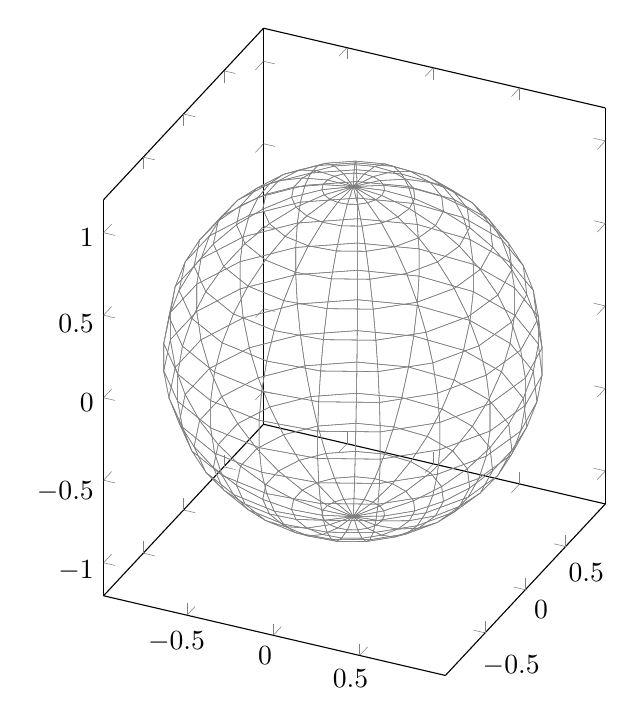
\begin{tikzpicture}
	\begin{axis}[
		axis equal image,
		%colormap/cool, % Cool colormap for better visualization
%		hide axis, % Optionally hide axis for a cleaner look
%		view={135}{30}, % Adjust the view angle
		]
		% Main spherical surface
		\addplot3[
		very thin,
		mesh,
        gray,
		samples=20, % Increased samples for smoother rendering
		domain=0:360, % Phi (longitude-like angle)
		y domain=0:180, % Theta (latitude-like angle)
		] 
		(
		{sin(y)*cos(x)}, % x = sin(theta)*cos(phi)
		{sin(y)*sin(x)}, % y = sin(theta)*sin(phi)
		{cos(y)}         % z = cos(theta)
		);
		
%		% Add gray polar grid (latitude lines)
%		\addplot3[
%		gray,
%		samples=20,
%		domain=0:360,
%		y domain=0:180,
%		] 
%		(
%		{sin(y)*cos(x)},
%		{sin(y)*sin(x)},
%		{cos(y)}
%		);
%		
%		% Longitude lines (azimuthal)
%		\foreach \phi in {0,30,...,330} { % Adjust step for density
%			\addplot3[
%			gray,
%			samples=20,
%			domain=0:180,
%			]
%			(
%			{sin(x)*cos(\phi)},
%			{sin(x)*sin(\phi)},
%			{cos(x)}
%			);
%		}
	\end{axis}
\end{tikzpicture}
	
\end{document}
